\documentclass[simplex.tex]{subfiles}
% NO NEED TO INPUT PREAMBLES HERE
% packages are inherited from simplex.tex; you can compile this on its own

\onlyinsubfile{
\title{NeuroData SIMPLEX Report: Subfile}
}

\begin{document}
\onlyinsubfile{
\maketitle
\thispagestyle{empty}

The following report documents the progress made by the labs of Randal~Burns and Joshua~T.~Vogelstein at Johns Hopkins University towards goals set by the DARPA SIMPLEX grant.

%%%% Table of Contents
\tableofcontents

%%%% Publications
\bibliographystyle{IEEEtran}
\begin{spacing}{0.5}
\section*{Publications, Presentations, and Talks}
\vspace{-20pt}
\nocite{*}
{\footnotesize	\bibliography{simplex}}
\end{spacing}
%%%% End Publications
}


\subsection{meda}

Matrix Exploratory Data Analysis (meda) is a package being developed to
allow for easy generation of modern summary statistics effective for
high-dimensional data analysis. 

\begin{itemize}
  \item Source code: \href{https://github.com/neurodata/meda}{https://github.com/neurodata/meda}
  \item Example output generated from Fisher's Iris data is here:
    \href{http://docs.neurodata.io/meda}{http://docs.neurodata.io/meda}
\end{itemize}

The goal of this package is to realize the following checklist:

\begin{spacing}{0.5}
{\footnotesize
{\large Given a new set of n samples of vectors in $\mathbb{R}^d$.}
\begin{enumerate}
  \item histogram of feature types (binary, integer, non-negative, character, string etc.)
  \item \# NaNs per row? Per column? Infs per row? Per column? "Zero" variance rows? columns?
\end{enumerate}

{\large For Level 0}
\begin{enumerate}
  \item Heat map of raw data that fits on screen (k-means++ to select 1000 samples, CUR to select 100 dimensions)
  \item 1st moment statistics
  \begin{enumerate}
    \item mean (line plot + heatmap)
    \item median (line plot + heatmap)
  \end{enumerate}
  \item 2nd moment statistics
  \begin{enumerate}
    \item correlation matrix (heatmap)
    \item matrix of energy distances (heatmap)
  \end{enumerate}
  \item density estimate
  \begin{enumerate}
    \item 1D marginals (Violin + jittered scatter plot of each dimension,  if n > 1000 or d>10, density heatmaps)
    \item 2D marginals (Pairs plots for top ~8 dimensions, if n*d>8000, 2D heatmaps)
  \end{enumerate}
  \item Outlier plot 
  \item cluster analysis (IDT++)
  \begin{enumerate}
    \item BIC curves
    \item mean line plot
    \item covariance matrix heatmaps
  \end{enumerate}
  \item spectral analysis
  \begin{enumerate}
    \item cumulative variance (with elbows) of data matrix
    \item eigenvectors (pairs plot + heatmap)
  \end{enumerate}
\end{enumerate}

{\large Iterate on results of mclust++ for each level, up to level 5 or so}
\begin{enumerate}
  \item heatmap, sorted by child node
  \item 1st order stats per child + difference between children
  \item 1st order stats per child + difference between children
  \item density estimate per child
  \begin{enumerate}
    \item 1D marginals: violion plot, separated by child node
    \item 2D marginals: pairs plots, color coded by cluster, voronoi diagram overlaid
  \end{enumerate}
  \item outlier plot for each child node
  \item cluster analysis per child
  \item spectral analysis per child
\end{enumerate}

{\large Scaling Options}
\begin{itemize}
  \item raw
  \item linear options
  \begin{itemize}
    \item linear squash between 0 \& 1
    \item mean subtract and standard deviation divide
    \item median subtract and median absolute deviation divide
    \item make unit norm
  \end{itemize}
  \item nonlinear
  \begin{itemize}
    \item rank
    \item sigmoid squash
  \end{itemize}
\end{itemize}

{\large robust options}
\begin{itemize}
  \item use \href{http://projecteuclid.org/euclid.bj/1438777595}{Geometric median and robust estimation in Banach spaces} 
    to obtain robust estimates of 1st and 2nd moments
\end{itemize}

{\large if features have categories}
\begin{enumerate}
  \item sort by category
  \item color code labels by category
\end{enumerate}

{\large if points have categories}
\begin{enumerate}
  \item label points in scatter plots by symbol
\end{enumerate}
}
\end{spacing}

\subsubsection{Synaptome Statistics}

We have continued to examine the Kristina15 synaptome dataset and have
now added the Weiler Chessboard dataset to our explorations.  Using 
\verb+meda+, and other methods along the way, we have started to compare
the structure of these two datasets, see figure~\ref{fig:synClaw}.  

\begin{figure}[h!]
\begin{cframed}
\centering
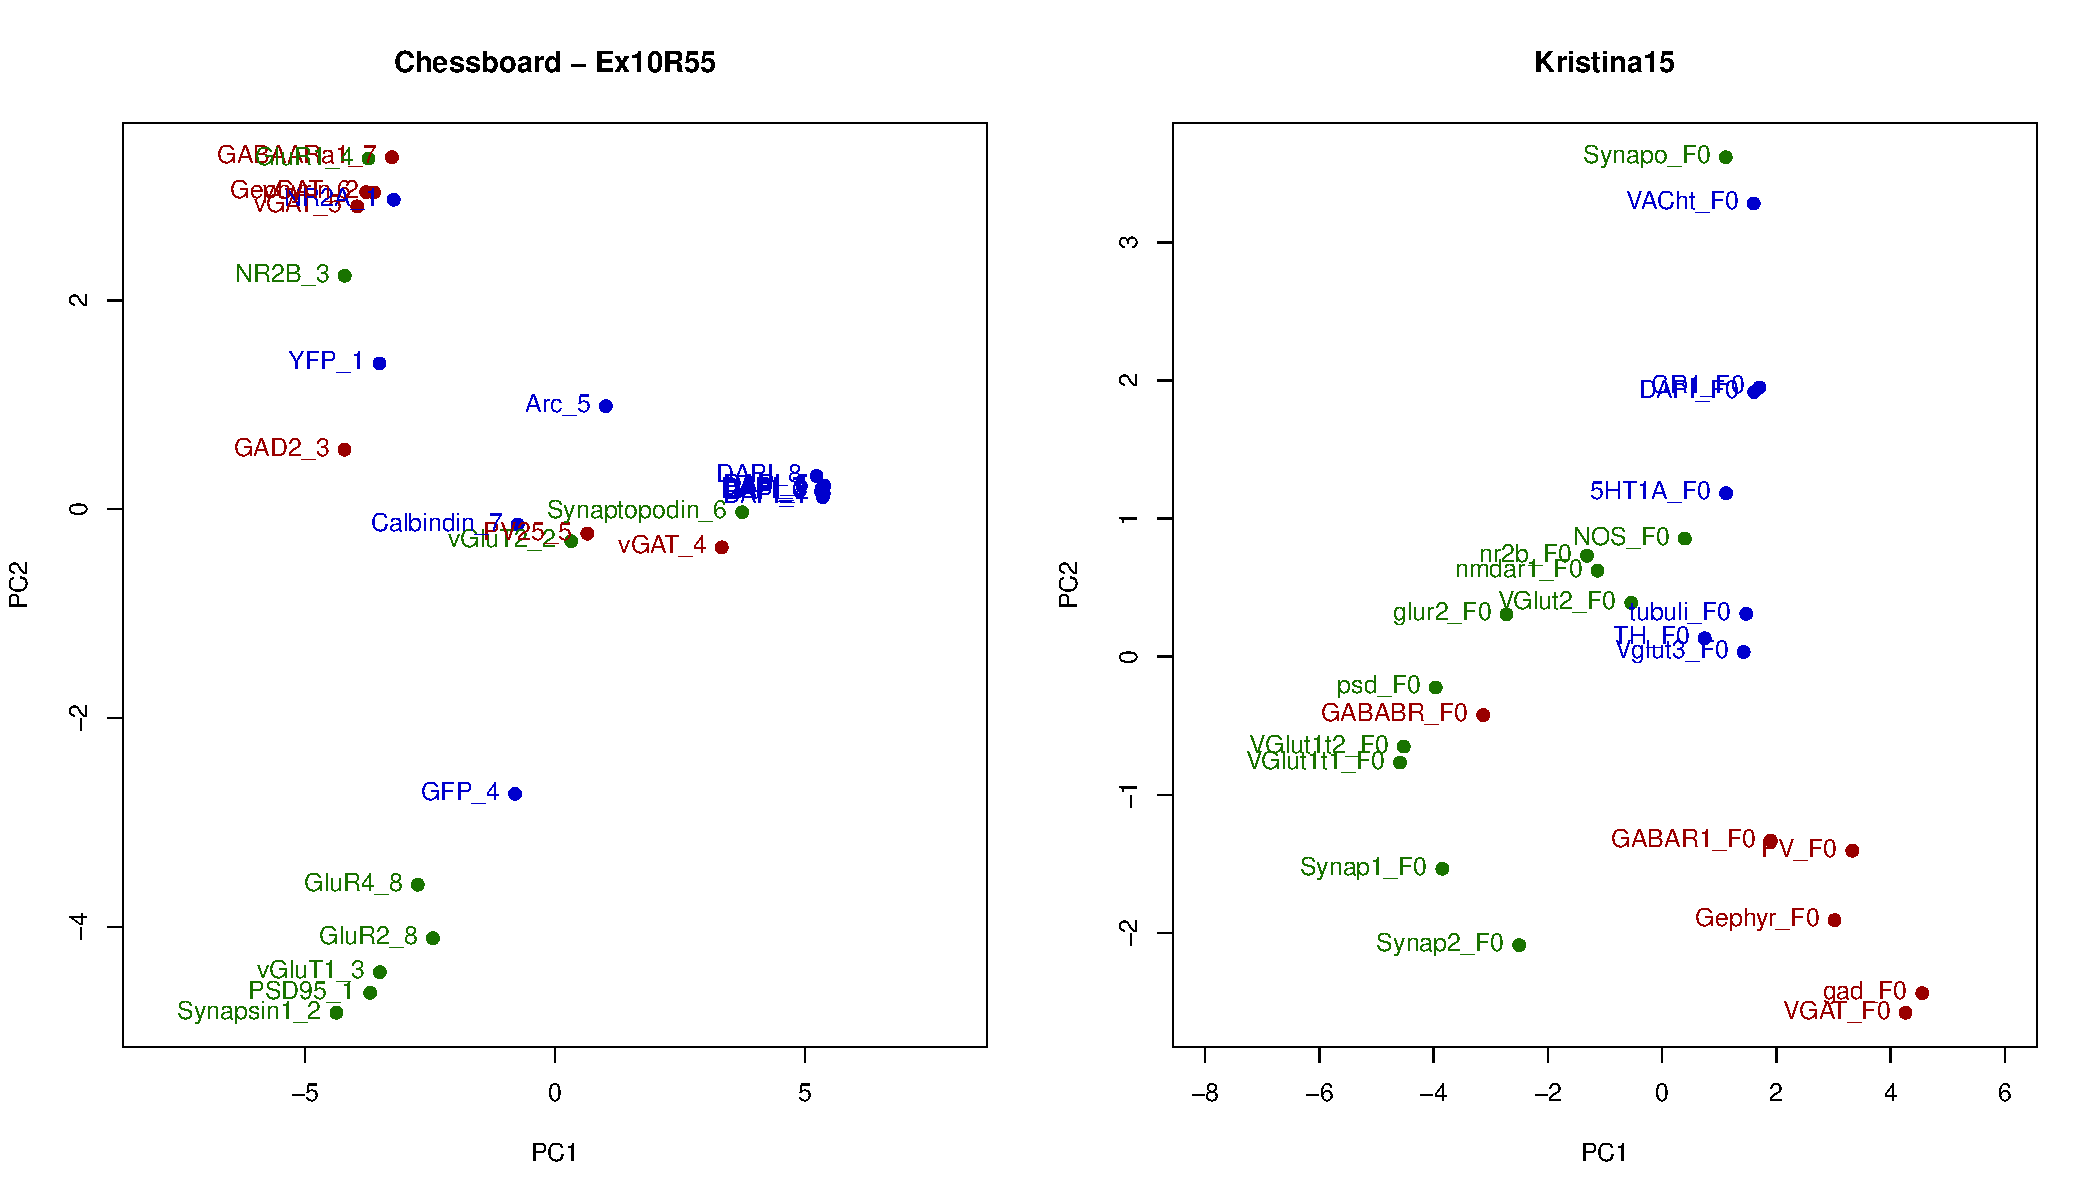
\includegraphics[width=\textwidth]{./figs/2dProjClaw.pdf}
\caption{
  Principal Component Analysis (PCA) has been run on the correlation
  matrices of both of these dataset respectively.  The first two
  principal components are plotted against each other.  The colors
  correspond to the type of marker, (``excitatory'' -- green,
  ``inhibitory'' -- red, ``other'' -- blue).  Notice that some markers are
  different between datasets, but there is a similar "claw" structure
  present. 
}
\label{fig:synClaw}
\end{cframed}
\end{figure}

\end{document}
